\section{Constitutive Laws}
\subsection*{RVE: Representative Volume Element}
\smallskip

A representative volume element (RVE) that can be related to a point $\underline{\mathbf{x}}$ must be approximately 10x smaller than the structure to be characterised and 10x larger than a typical length of the underlying mesostructure. In periodic materials, the generating \textbf{unit cell} (UC) can be considered as a RVE, provided that: $RVE = 10 \cdot UC$ \\

\columnbreak
\subsection*{Standard generalised material}
$\tensor[^{nom}]{\psi}{} (\underline{x},t) = \tensor[^{nom}]{\psi}{} (\underline{x}, \underline{\underline{F}}, T, \zeta_1, \zeta_2, ..., \zeta_n)$ \qquad Free energy \\
$ \tensor[^{nom}]{\phi}{} (\underline{x},t) = \tensor[^{nom}]{\phi}{} (\underline{x}, \underline{\underline{\dot{F}}}, \dot{T}, \dot{\zeta_1}, \dot{\zeta_2}, ..., \dot{\zeta_n})$ \qquad Dissipation potential \\

\textbf{Objective constitutive laws} $\Leftrightarrow$ \textbf{Material frame indifference} \\
Constitutive relationships expressed in \textbf{objective} variables of state, i.e. formulated in material variables that are invariant under a rigid body motion:

$\psi (\underline{x},t) = \psi (\underline{x}, \underline{\underline{E}}, T, \chi_1, \chi_2, ..., \chi_n)$ \hspace{15.6mm}Free energy \\
$ \phi (\underline{x},t) = \phi (\underline{x}, \underline{\underline{\dot{E}}}, \dot{T}, \dot{\chi_1}, \dot{\chi_2}, ..., \dot{\chi_n}, \frac{\underline{q}}{T})$ \hspace{11.1mm} Dissipation potential\\

Inconvenience of not using variables that are directly accessible from experiments! (e.g. $\underline{\underline{\mathbf{P}}}, \underline{\underline{\mathbf{F}}}$). \\


\subsection*{Heterogeneity and anisotropy}
\textbf{Heterogeneity:} variable $\underline{\mathbf{x}}$ in the constitutive laws express the heterogeneous aspect of the body that exhibit distinct properties as a function of position. \\
\textbf{Anisotropy:} based upon the notion of symmetry that expresses an invariance with respect to certain operations. Symmetry allows simplification of the mathematical formulation of the constitutive laws.

\begin{itemize}
\item \underline{Crystallographic groups of symmetry} (triclinic, monoclinic, tetragonal, trigonal, hexagonal, cubic, ...)
\item \underline{Isotropic:} infinity of axes of rotation of an infinite nature
\item \underline{Transverse isotropic:} one axis of rotation of infinite nature
\end{itemize}

\subsection*{Conservative laws}
Conservative constitutive laws include \textbf{storage} but \textbf{no dissipation of energy} and describe therefore \textbf{fully reversible} processes $(\phi \equiv 0)$. \\
\textbf{Elasticity:} generally monotonic and formulated by means of invertible functions, loading and unloading paths are perfectly superimposed. Conservative laws that depend exclusively on the total deformation. \\
Generally, elastic functions are not linear:
$ \underline{\underline{S}} (\alpha \underline{\underline{E}}) \neq \alpha \underline{\underline{S}} (\underline{\underline{E}}) $ \\
\textbf{Linear Elasticity:} $S(E) = \epsilon E$ Hook's Law, with $\epsilon$: elastic modulus, $E$: strain. \\
Free energy potential: $\Psi(E)=\frac{1}{2}\epsilon E^2$

\begin{center}
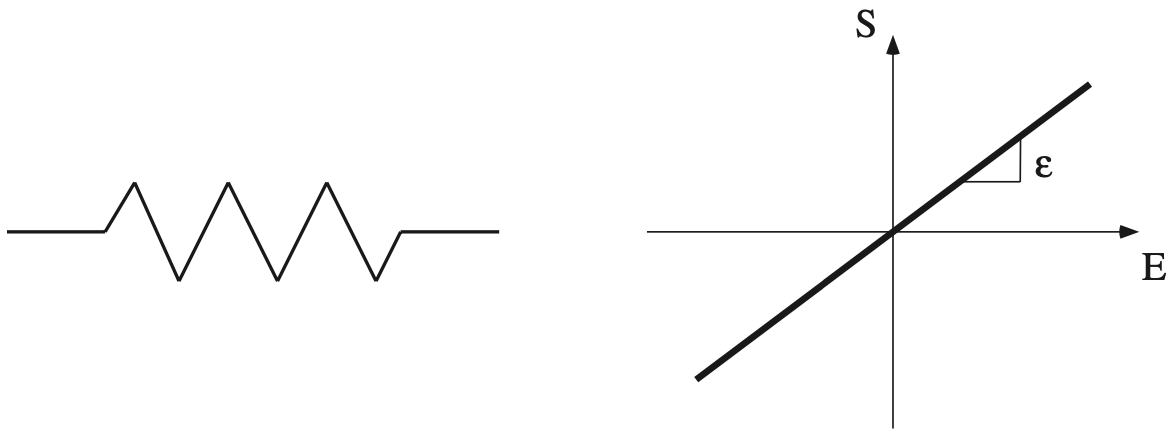
\includegraphics[width=0.5\linewidth]{img/Lin} \\
\end{center}

\textbf{Nonlinear Elasticity:} Elastic and monotone constitutive law \\ $\rightarrow$ material non-linearity.
$S(E) = \frac{\epsilon}{3}\left(\frac{\sqrt{2E + 1}-1}{2E + 1})+2E\right)$
\begin{center}
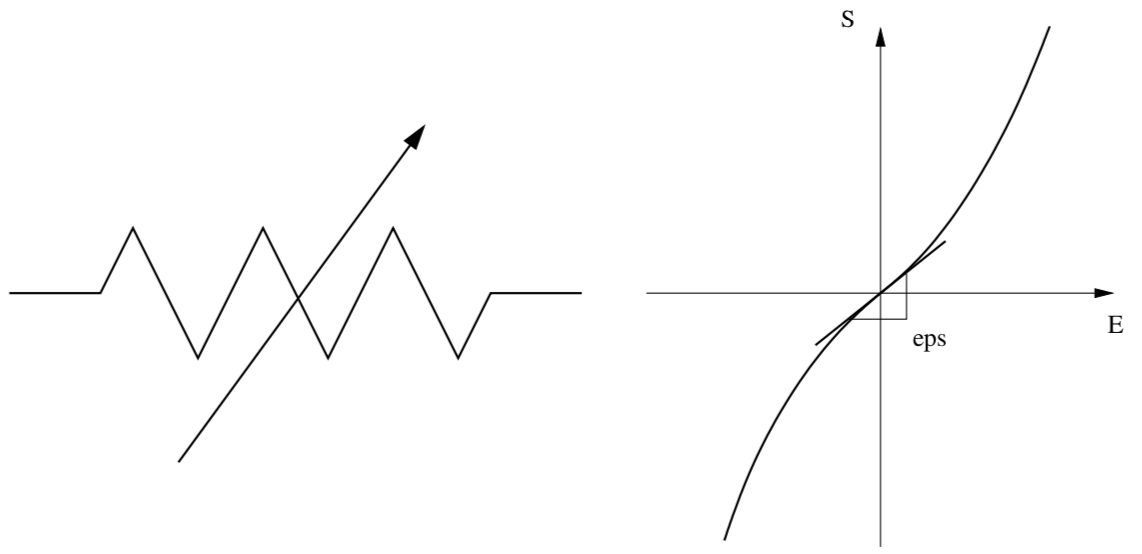
\includegraphics[width=0.5\linewidth]{img/NonLin} \\
\end{center}
\textbf{Geometrical nonlinearity:} linear law with respect to the objective variables is not linear in the nominal variables. \\
$ P(H) = \frac{\epsilon}{2} H (H+1) (H+2)$ induced by the use of material variables! \\

\textbf{Piecewise linear elasticity:} material behaviour law with an elastic modulus that differs in tension and compression.

$S(E) =$
$\begin{cases} 
\epsilon_{-}E, & E \leqslant 0 \\ \epsilon_{+}E, & E \geqslant 0
\end{cases}$

\begin{center}
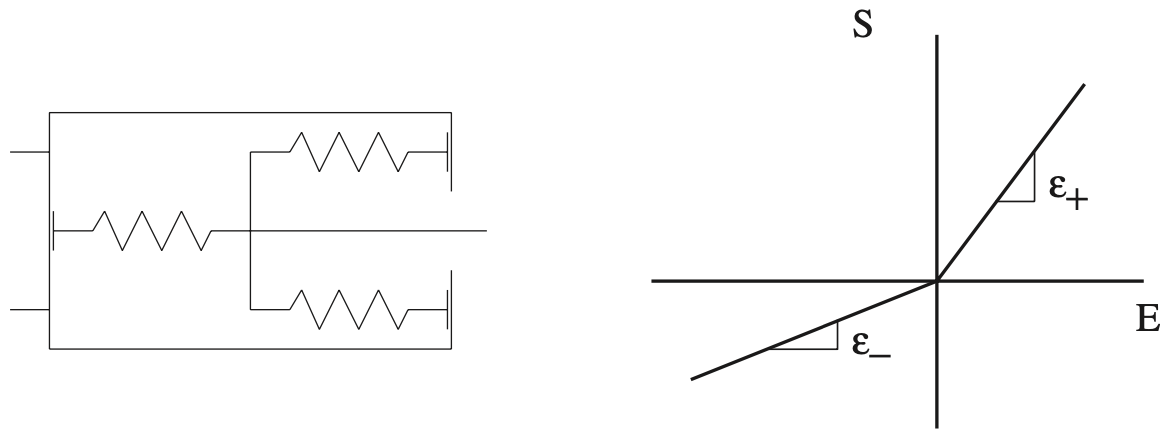
\includegraphics[width=0.5\linewidth]{img/PiecLin} \\
\end{center}



\subsection*{Nonconservative laws}
Cannot be derived from a free energy potential $\rightarrow$ irreversible \\
$\phi \neq 0$ (non-zero dissipation potential). Loading and unloading paths cannot be superimposed in a stress-strain diagram.\\

\textbf{Viscoelasticity:} \\
In Kelvin model, strain remains the only state variable and the total stress is the sum of conservative and dissipative contributions. \\
$\psi (E) = \frac{1}{2} \epsilon E^2$ \qquad $\phi (\dot{E}) =  \frac{1}{2} \mu \dot{E}^2 $ \quad $S(E,\dot{E}) = \epsilon E + \mu \dot{E} $ \\
Where $\epsilon$: elastic module, $\mu$: viscosity coeff. \\

The involved spring and dashpot are independently linear with respect to $E$ and $\dot{E}$, but the total stress is not bilinear with respect to the two variables because they are not independent in a historical sense. Linearity is composed of \textbf{homogeneity} and \textbf{additivity}.

\textbf{Elastoplasticity:} \\
Rate independent, linear elasto-plastic material behavior. Rheologic model: spring with a slider in series. The total deformation is decomposed in elastic+plastic parts.
$E = E^e + E^p$, leading to irreversible strains.

\begin{center}
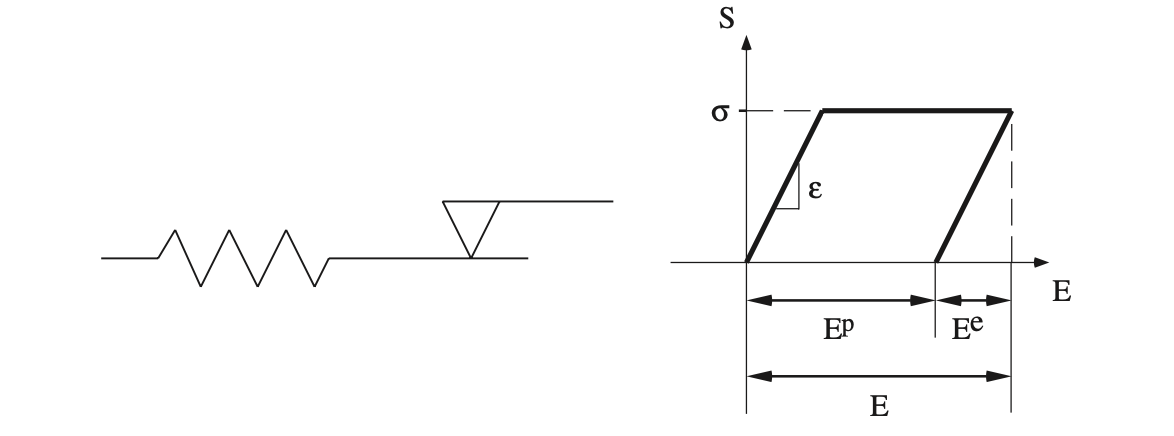
\includegraphics[width=0.5\linewidth]{img/ElastoPlast} \\
\end{center}

\textbf{Damage:} \\
A damaged material has a memory in form of a reduction of its elastic properties $\epsilon$ and can be modelled with the help of an internal variable D, that represents the relative surface occupied by defects or fissures. Elasticity of the tissue is altered but no residual deformation is accounted for. \\
Rheological model: $\tilde{S} = \frac{S}{1-D}$ \\
Corresponding stresses: $S (E,D) = \epsilon (1-D) E,$ \qquad $S^D (E,D) = \frac{1}{2} \epsilon E^2$

\begin{center}
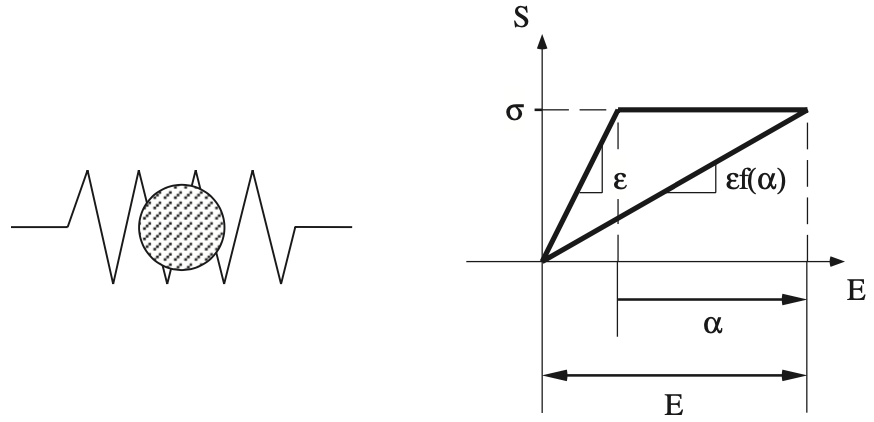
\includegraphics[width=0.5\linewidth]{img/Damage} \\
Rate independent perfect damage
\end{center}